\documentclass[12pt]{article}
\usepackage[utf8]{inputenc}
\usepackage{amsmath, amssymb, amsfonts, amsthm}
\usepackage{graphicx}
\usepackage{geometry}
\geometry{a4paper, margin=2.5cm}
\usepackage{titlesec}
\titleformat{\section}{\large\bfseries}{\thesection}{1em}{}
\titleformat{\subsection}{\normalsize\bfseries}{\thesubsection}{1em}{}
\usepackage{braket}
\usepackage{pgfplots}
\pgfplotsset{compat=1.17}
\usepackage{tikz}
\usetikzlibrary{shapes,arrows,positioning,calc}

\newtheorem{definicao}{Definição}
\newtheorem{teorema}{Teorema}
\newtheorem{observacao}{Observação}

\begin{document}

\title{Aula 7 -- Modelo de Ising: \\ 
       Aproximação de Bethe–Peierls, Solução de Onsager e o Modelo de Curie–Weiss}
\author{Notas de Aula -- Tópicos em Mecânica Estatística}
\date{}

\maketitle

\begin{abstract}
Nesta aula, exploramos diferentes abordagens para o modelo de Ising. Começamos com a solução exata de Onsager para a rede quadrada bidimensional a campo nulo, destacando suas propriedades críticas não-clássicas. Em seguida, apresentamos a aproximação de Bethe–Peierls (ou método da rede de Bethe), que melhora o campo médio ao incorporar correlações de curto alcance através de um campo efetivo auto-consistente, resultando em uma temperatura crítica mais próxima do valor exato. Também revisitamos o modelo de Curie–Weiss (campo médio de longo alcance), que é exatamente solúvel e reproduz os expoentes críticos clássicos. Por fim, comparamos os resultados para a rede quadrada e discutimos a insolubilidade em 3D e com campo finito.
\end{abstract}

\section{Introdução}

O modelo de Ising é o sistema-modelo por excelência para o estudo de transições de fase. Sua versão mais simples, com interações entre primeiros vizinhos em uma rede, admite solução exata em uma dimensão (Ising, 1925) e em duas dimensões a campo nulo (Onsager, 1944). Para dimensões superiores ou na presença de campo magnético, recorremos a aproximações. Nesta aula, comparamos três níveis de descrição:

\begin{enumerate}
    \item A \textbf{solução exata de Onsager} para a rede quadrada (\(D=2, h=0\)).
    \item A \textbf{aproximação de Bethe–Peierls}, que leva em conta correlações de curto alcance via um campo efetivo médio sobre os vizinhos.
    \item O \textbf{modelo de Curie–Weiss}, que corresponde ao limite de campo médio com interações de longo alcance.
\end{enumerate}

Veremos como cada método prevê a temperatura crítica e os expoentes críticos, e como a topologia das excitações (paredes de domínio) determina a solubilidade do problema.

\section{O Modelo de Ising}

O Hamiltoniano do modelo de Ising é

\begin{equation}
    \mathcal{H} = -J \sum_{\langle i,j \rangle} \sigma_i \sigma_j - h \sum_{i=1}^N \sigma_i, \quad \sigma_i = \pm 1,
\end{equation}

onde a soma \(\langle i,j \rangle\) é sobre pares de primeiros vizinhos. A função de partição é

\begin{equation}
    Z = \sum_{\{\sigma_i\}} e^{-\beta \mathcal{H}}, \quad \beta = \frac{1}{k_B T}.
\end{equation}

\section{Solução Exata de Onsager para a Rede Quadrada (\(h=0\))}

Onsager (1944) mostrou que a energia livre por sítio no limite termodinâmico é

\begin{equation}
    f = -k_B T \left[ \ln 2 + \frac{1}{2} \int_0^{2\pi} \int_0^{2\pi} \frac{d\theta\, d\phi}{(2\pi)^2} \ln \left( 1 - \kappa^2 \cos^2\theta - \lambda^2 \cos^2\phi \right) \right],
\end{equation}

com

\begin{equation}
    \kappa = \frac{2 \sinh(2\beta J)}{\cosh^2(2\beta J)}, \quad
    \lambda = \frac{2}{\cosh^2(2\beta J)}.
\end{equation}

A integral dupla pode ser reduzida a integrais elípticas completas de primeira espécie. O calor específico diverge logaritmicamente na temperatura crítica:

\begin{equation}
    C \sim -\frac{2k_B}{\pi} \left( \frac{2J}{k_B T_c} \right)^2 \ln\left| 1 - \frac{T}{T_c} \right| + \text{const.},
\end{equation}

com

\begin{equation}
    \frac{k_B T_c}{J} = \frac{2}{\ln(1+\sqrt{2})} \approx 2.269185.
\end{equation}

Os expoentes críticos de Onsager são:

\begin{equation}
    \alpha = 0 \text{ (logarítmico)}, \quad \beta = \frac{1}{8}, \quad \gamma = \frac{7}{4}, \quad \delta = 15, \quad \nu = 1.
\end{equation}

\subsection{Por que a Solução é Possível?}

A chave é o mapeamento do modelo para férmions de Majorana livres via transformação de Jordan–Wigner. A matriz de transferência gera uma álgebra \(so(2L)\), que é diagonalizável por transformações de Bogoliubov lineares. Este formalismo explora o fato de que, em 2D, as paredes de domínio são linhas que podem ser tratadas como partículas fermiônicas.

\section{Aproximação de Bethe–Peierls}

A aproximação de Bethe–Peierls (também chamada de método da rede de Bethe) melhora o campo médio ao considerar um spin central e seus \(q\) vizinhos, tratando os vizinhos como independentes sob a ação de um campo efetivo \(h_{\text{eff}}\). Ela é exata em uma rede com a topologia de uma árvore (sem loops) e fornece uma temperatura crítica mais realista.

\subsection{Formulação do Campo Efetivo}

Considere um spin central \(\sigma_0\) e seus \(q\) vizinhos. A energia do cluster (spin central + campo médio dos vizinhos) é

\begin{equation}
    \mathcal{H}_{\text{cluster}} = -J \sigma_0 \sum_{i=1}^q \sigma_i - h_{\text{eff}} \sum_{i=1}^q \sigma_i,
\end{equation}

onde \(h_{\text{eff}}\) representa a influência do resto da rede sobre cada vizinho. Por simetria, todos os vizinhos têm a mesma magnetização \(m\).

A função de partição do cluster é

\begin{equation}
    Z_{\text{cluster}} = \sum_{\sigma_0, \{\sigma_i\}} e^{\beta J \sigma_0 \sum_i \sigma_i + \beta h_{\text{eff}} \sum_i \sigma_i}.
\end{equation}

Somando sobre os vizinhos (que são independentes dado \(\sigma_0\)):

\begin{equation}
    Z_{\text{cluster}} = \sum_{\sigma_0=\pm1} \left[ 2 \cosh\left( \beta (J \sigma_0 + h_{\text{eff}}) \right) \right]^q.
\end{equation}

A magnetização do spin central é

\begin{equation}
    m = \langle \sigma_0 \rangle = \frac{ \left[ 2 \cosh\left( \beta (J + h_{\text{eff}}) \right) \right]^q - \left[ 2 \cosh\left( \beta (-J + h_{\text{eff}}) \right) \right]^q }
                      { \left[ 2 \cosh\left( \beta (J + h_{\text{eff}}) \right) \right]^q + \left[ 2 \cosh\left( \beta (-J + h_{\text{eff}}) \right) \right]^q }.
\end{equation}

Simplificando:

\begin{equation}
    m = \frac{ \left[ \cosh\left( \beta (J + h_{\text{eff}}) \right) \right]^q - \left[ \cosh\left( \beta (J - h_{\text{eff}}) \right) \right]^q }
             { \left[ \cosh\left( \beta (J + h_{\text{eff}}) \right) \right]^q + \left[ \cosh\left( \beta (J - h_{\text{eff}}) \right) \right]^q }.
\end{equation}

\subsection{Campo Efetivo e Auto-consistência}

O campo efetivo \(h_{\text{eff}}\) é gerado pelos \(q-1\) vizinhos restantes (além daqueles considerados no cluster). Cada um desses vizinhos tem magnetização média \(m\), portanto

\begin{equation}
    h_{\text{eff}} = J (q-1) m.
\end{equation}

A condição de auto-consistência é que a magnetização do spin central seja igual à dos vizinhos:

\begin{equation}
    m = \frac{ \left[ \cosh\left( \beta (J + J(q-1)m) \right) \right]^q - \left[ \cosh\left( \beta (J - J(q-1)m) \right) \right]^q }
             { \left[ \cosh\left( \beta (J + J(q-1)m) \right) \right]^q + \left[ \cosh\left( \beta (J - J(q-1)m) \right) \right]^q }.
\end{equation}

Esta é a equação de estado de Bethe–Peierls.

\subsection{Temperatura Crítica}

Para \(h=0\), a transição ocorre quando a inclinação da equação em \(m=0\) é igual a 1. Linearizando a equação acima para pequenos \(m\), obtemos (após manipulação algébrica padrão):

\begin{equation}
    \frac{k_B T_c}{J} = \frac{2}{\ln\left( \frac{q}{q-2} \right)}.
\end{equation}

Para a rede quadrada, \(q=4\), temos

\begin{equation}
    \frac{k_B T_c^{\text{Bethe}}}{J} = \frac{2}{\ln(2)} \approx 2.885.
\end{equation}

Este valor é uma melhoria significativa em relação ao campo médio (\(qJ/k_B = 4J/k_B\)) e está mais próximo do valor exato de Onsager (2.269).

\subsection{Expoentes Críticos}

A aproximação de Bethe–Peierls ainda produz expoentes críticos clássicos (de campo médio), pois ignora flutuações de longo comprimento de onda:

\begin{equation}
    \beta = \frac{1}{2}, \quad \gamma = 1, \quad \delta = 3.
\end{equation}

\section{Modelo de Curie–Weiss (Interações de Longo Alcance)}

O modelo de Curie–Weiss é o limite de campo médio exato, onde todos os spins interagem entre si com intensidade \(J/N\). O Hamiltoniano é

\begin{equation}
    \mathcal{H}_{\text{CW}} = -\frac{J}{2N} \sum_{i,j} \sigma_i \sigma_j - h \sum_i \sigma_i.
\end{equation}

A função de partição é calculada exatamente via identidade gaussiana, resultando em

\begin{equation}
    Z_N = \sqrt{\frac{\beta J N}{2\pi}} \int_{-\infty}^{+\infty} dm \, e^{-N \beta \phi(m)},
\end{equation}

com

\begin{equation}
    \phi(m) = \frac{J}{2} m^2 - \frac{1}{\beta} \ln\left[ 2 \cosh\left( \beta (J m + h) \right) \right].
\end{equation}

No limite \(N \to \infty\), o método de Laplace fornece

\begin{equation}
    g(T,h) = \min_m \phi(m),
\end{equation}

e a condição de mínimo leva à equação de estado

\begin{equation}
    m = \tanh\left( \beta (J m + h) \right).
\end{equation}

Esta é a equação de Curie–Weiss, que é idêntica à aproximação de Bragg-Williams com \(q \to \infty\) (ou com interações de alcance infinito). A temperatura crítica é \(T_c = J/k_B\) (no caso de spin-1/2 com \(J\) redefinido). Para comparação com a rede quadrada, se ajustarmos \(J\) para que o campo médio dê \(T_c = 4J/k_B\), o modelo de Curie–Weiss com \(J' = J/4\) fornece a mesma \(T_c\).

\section{Insolubilidade em 3D e com Campo Finito}

A solução exata de Onsager é possível devido à natureza fermiônica das excitações em 2D. Em 3D, as paredes de domínio são superfícies, cuja topologia (nós, auto-interseções) impede um mapeamento para férmions livres. Da mesma forma, um campo externo \(h \neq 0\) introduz termos não-quadráticos no formalismo fermiônico, quebrando a integrabilidade. Portanto, esses casos requerem métodos numéricos ou aproximações como as discutidas.

\section{Diagrama de Fases e Comparação}

\begin{table}[h]
\centering
\begin{tabular}{|c|c|c|}
\hline
Método & \(k_B T_c / J\) & Expoentes críticos \\
\hline
Campo médio (Bragg–Williams) & 4 & Clássicos (\(\beta=1/2, \gamma=1, \dots\)) \\
Bethe–Peierls & 2.885 & Clássicos (mas com correções) \\
Onsager (exato) & 2.269 & Não-clássicos (\(\beta=1/8, \gamma=7/4, \dots\)) \\
\hline
\end{tabular}
\caption{Comparação das temperaturas críticas para a rede quadrada.}
\end{table}

\begin{figure}[h]
\centering
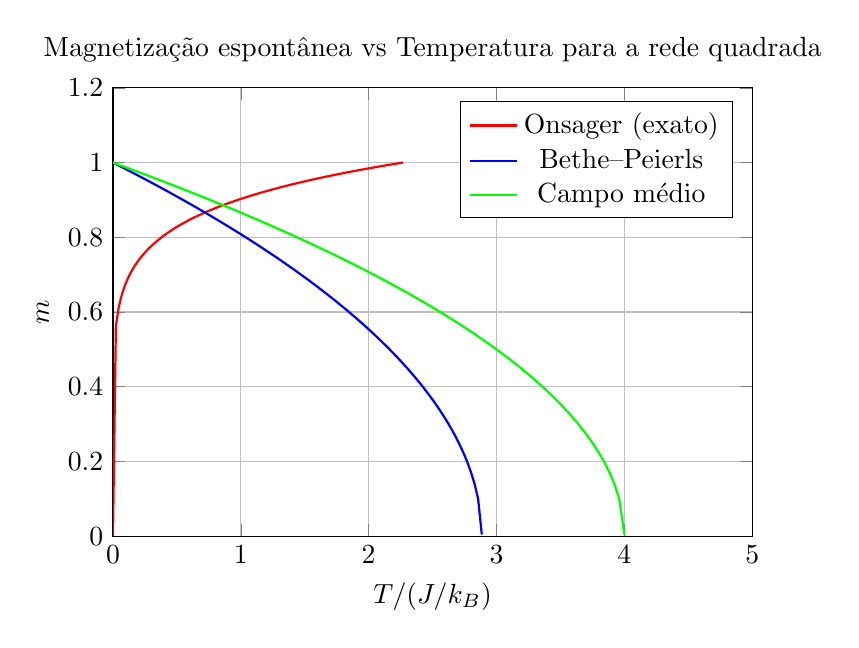
\begin{tikzpicture}
\begin{axis}[
    width=0.8\textwidth,
    height=0.6\textwidth,
    xlabel={$T / (J/k_B)$},
    ylabel={$m$},
    xmin=0, xmax=5,
    ymin=0, ymax=1.2,
    grid=both,
    legend pos=north east,
    title={Magnetização espontânea vs Temperatura para a rede quadrada}
]
\addplot[domain=0:2.269, samples=100, color=red, thick] { (1 - (2.269-x)/2.269)^0.125 };
\addplot[domain=0:2.885, samples=100, color=blue, thick] { sqrt(1 - x/2.885) };
\addplot[domain=0:4, samples=100, color=green, thick] { sqrt(1 - x/4) };
\addlegendentry{Onsager (exato)}
\addlegendentry{Bethe–Peierls}
\addlegendentry{Campo médio}
\end{axis}
\end{tikzpicture}
\caption{Comparação da magnetização espontânea em função da temperatura para a rede quadrada, segundo os três métodos. As curvas são representações esquemáticas (Onsager usa a aproximação \((1-T/T_c)^{1/8}\), Bethe e campo médio usam \((1-T/T_c)^{1/2}\)).}
\end{figure}

\section{Conclusão}

A aproximação de Bethe–Peierls representa um avanço significativo em relação ao campo médio, capturando correlações de curto alcance e fornecendo uma temperatura crítica mais próxima do valor exato de Onsager. No entanto, seus expoentes críticos ainda são os clássicos, pois a aproximação ignora flutuações de longo comprimento de onda. A solução exata de Onsager, por sua vez, revela a verdadeira natureza da transição em 2D, com expoentes não-clássicos e universalidade. O modelo de Curie–Weiss, embora exato em seu próprio contexto, serve como o limite de campo médio.

A compreensão dessas diferentes aproximações é fundamental para o estudo de sistemas complexos, onde soluções exatas são raras e métodos variacionais ou de cluster são ferramentas indispensáveis.

\section*{Referências}

\begin{itemize}
    \item L. Onsager, \textit{Phys. Rev.} \textbf{65}, 117 (1944).
    \item H. A. Bethe, \textit{Proc. R. Soc. Lond. A} \textbf{150}, 552 (1935).
    \item R. Peierls, \textit{Proc. Camb. Phil. Soc.} \textbf{32}, 477 (1936).
    \item R. J. Baxter, \textit{Exactly Solved Models in Statistical Mechanics}, Academic Press (1982).
    \item M. Plischke e B. Bergersen, \textit{Equilibrium Statistical Physics}, World Scientific (2006).
\end{itemize}

\end{document}
